\section{Design}

\subsection{Architectural Design}


\begin{figure}[htb]
\centering
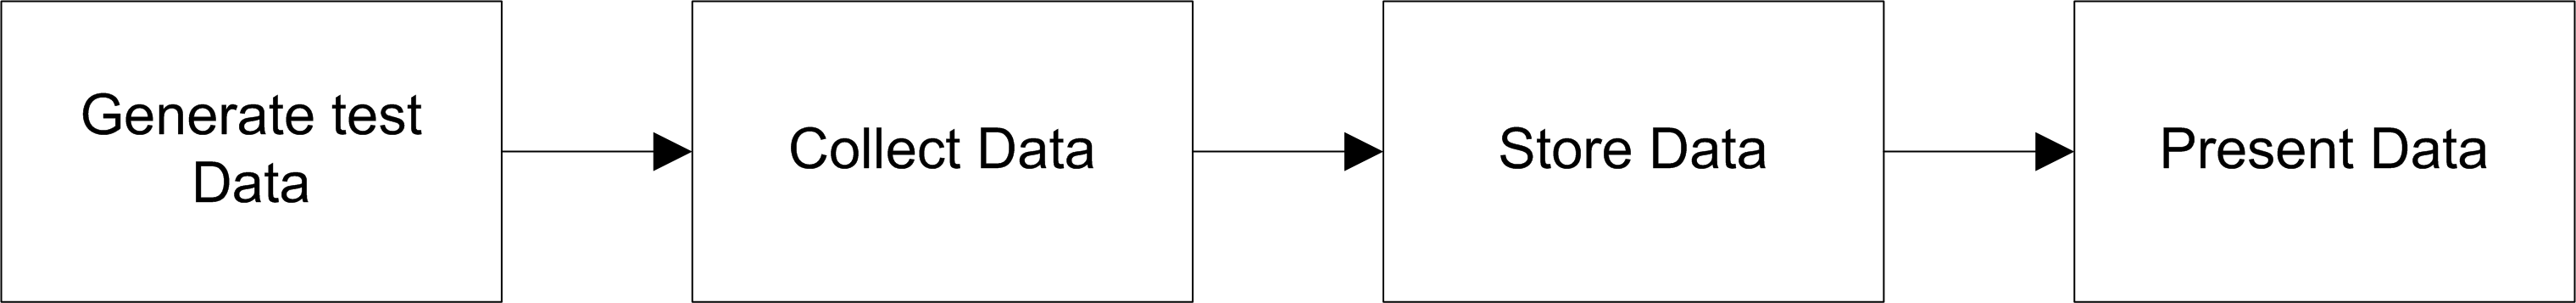
\includegraphics[width=0.8\textwidth]{img/3yp-arch.png}
\caption{Solution Architecture showing Data Flow}
\label{fig:arch}
\end{figure}


\begin{figure}[htb]
\centering
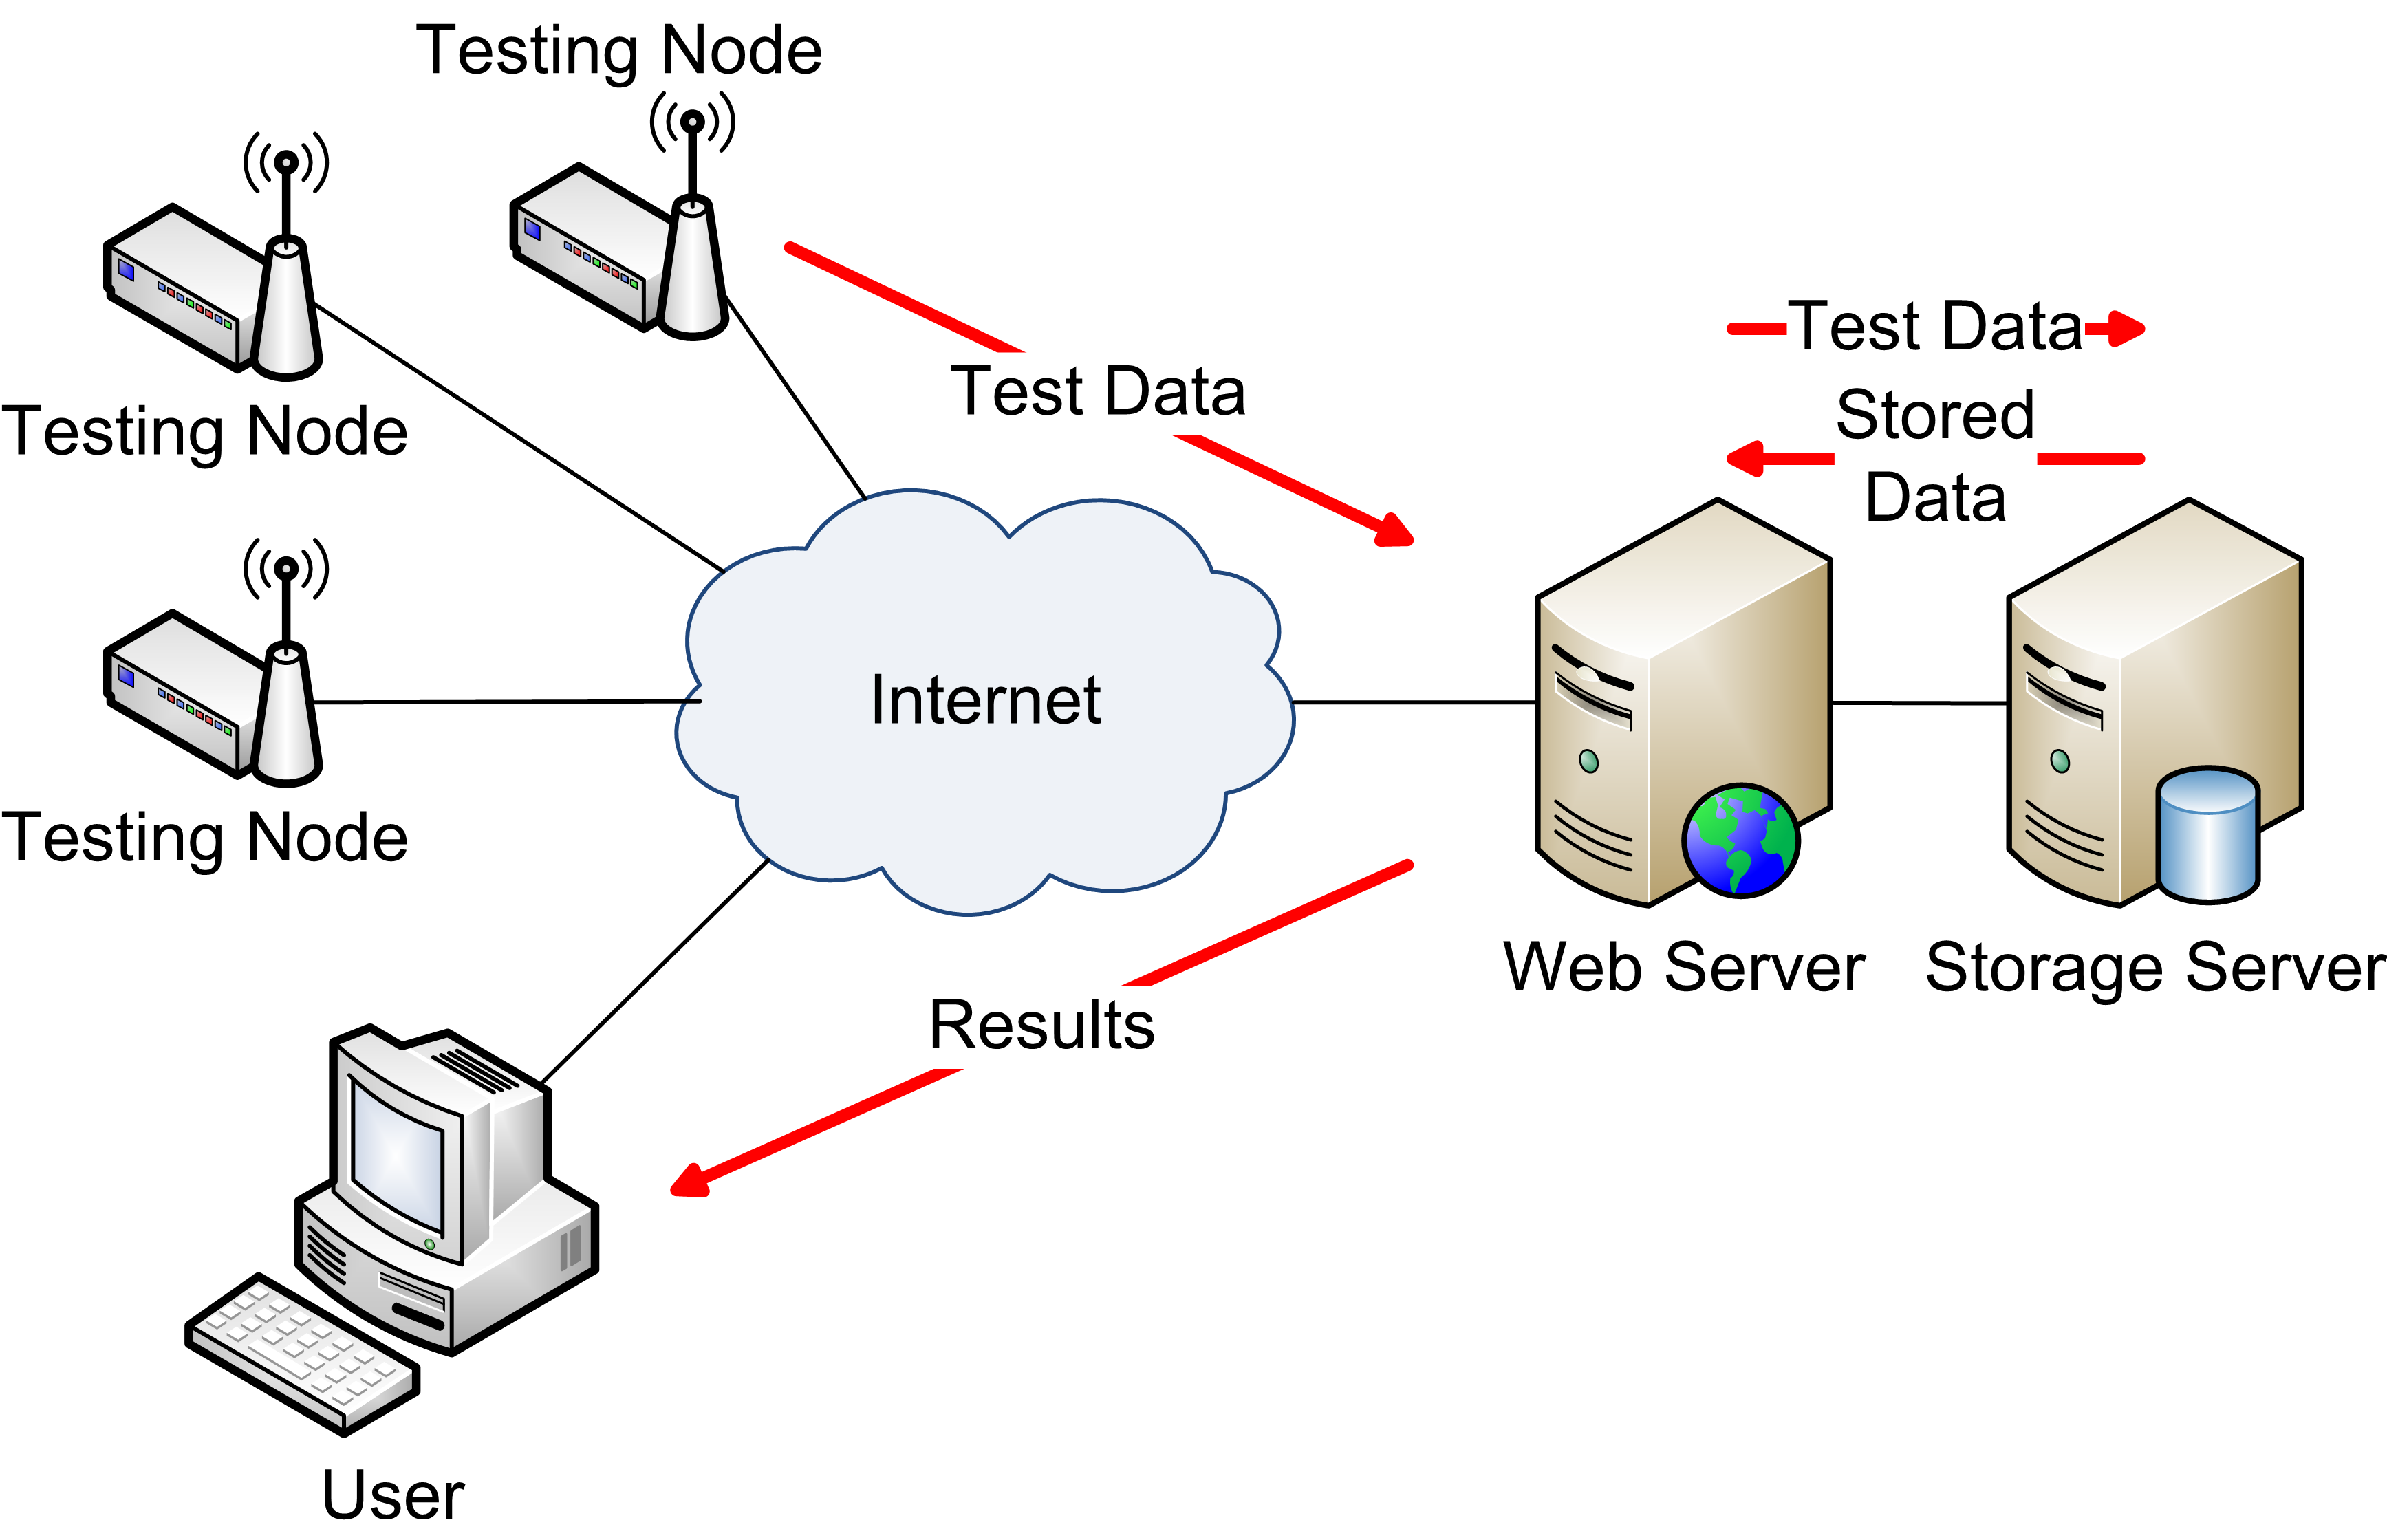
\includegraphics[width=0.7\textwidth]{img/3yp-phys.png}
\caption{Example of Physical Component Structure}
\label{fig:phys}
\end{figure}

\subsection{Detailed Design}

\nomenclature{SSL}{Secure Sockets Layer}
\nomenclature{HTTP}{Hypertext Transfer Protocol}
\nomenclature{REST}{Representational state transfer architecture} 

\begin{figure}[htb]
\centering
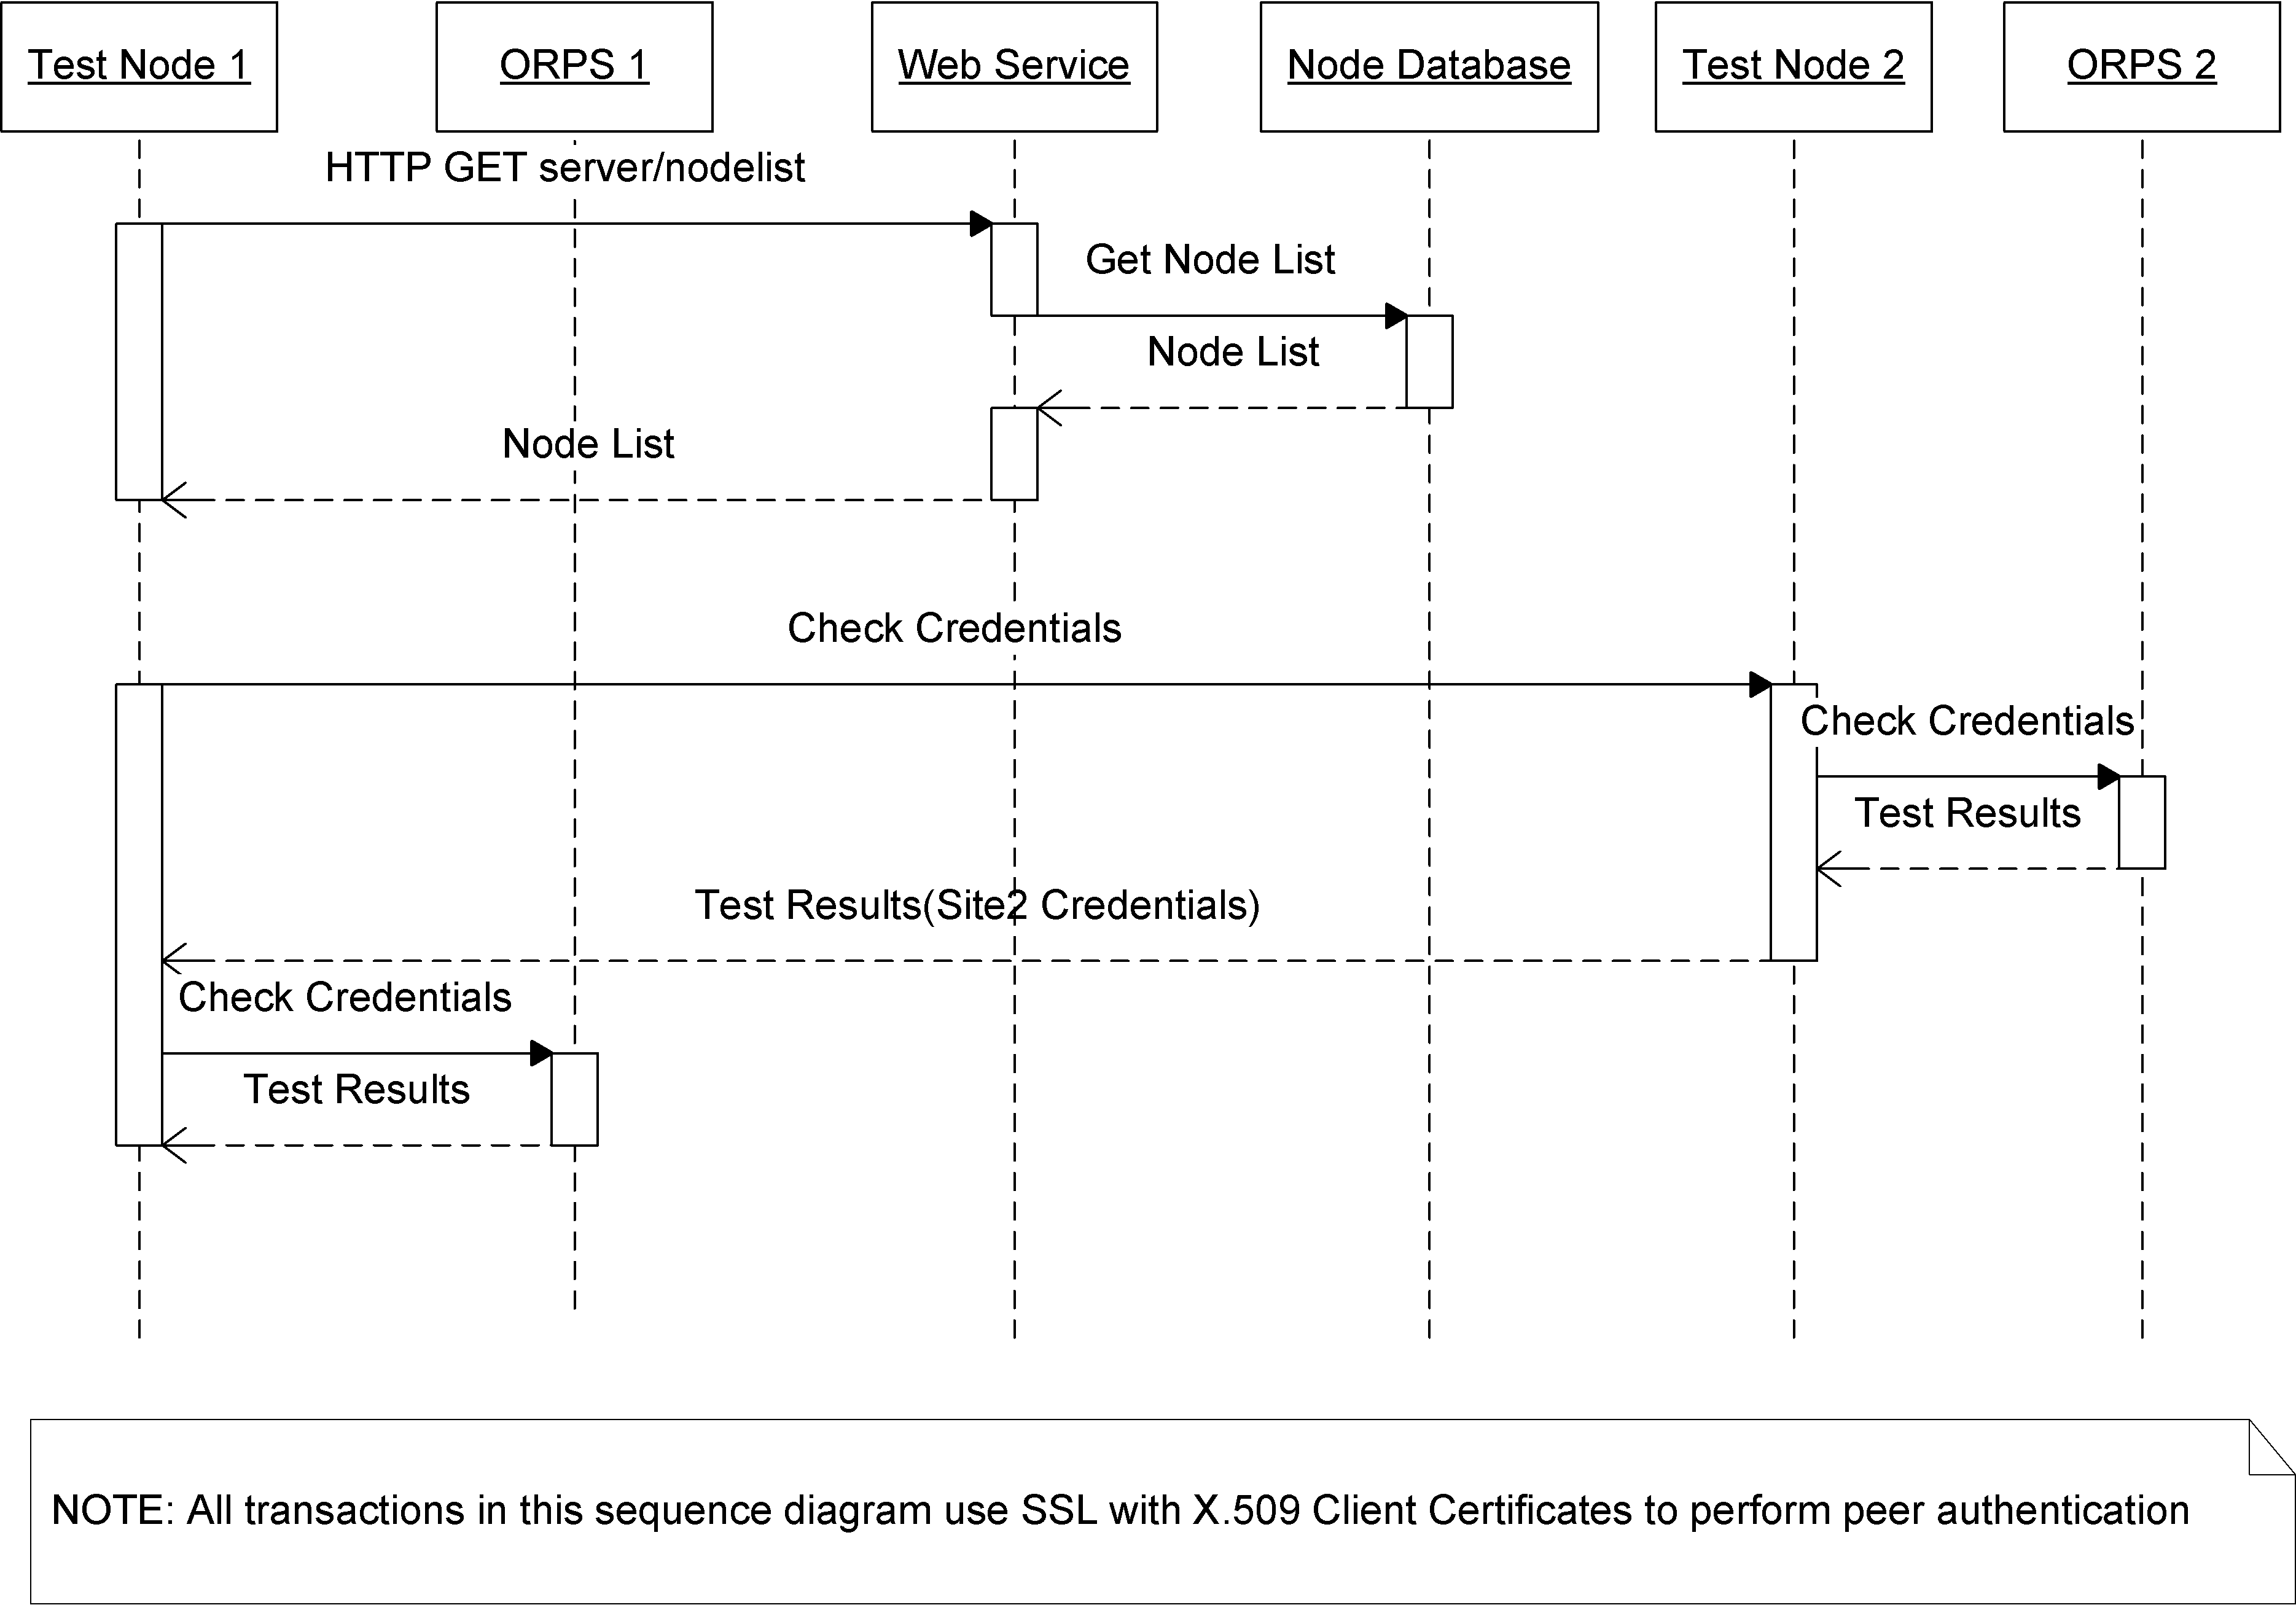
\includegraphics[width=0.7\textwidth]{img/sec-struct-sequence.png}
\caption{UML Sequence Diagram of Credential Exchange}
\label{fig:sec-seq}
\end{figure}
\nomenclature{UML}{Unified Modeling Language}

\begin{figure}[htb]
\centering
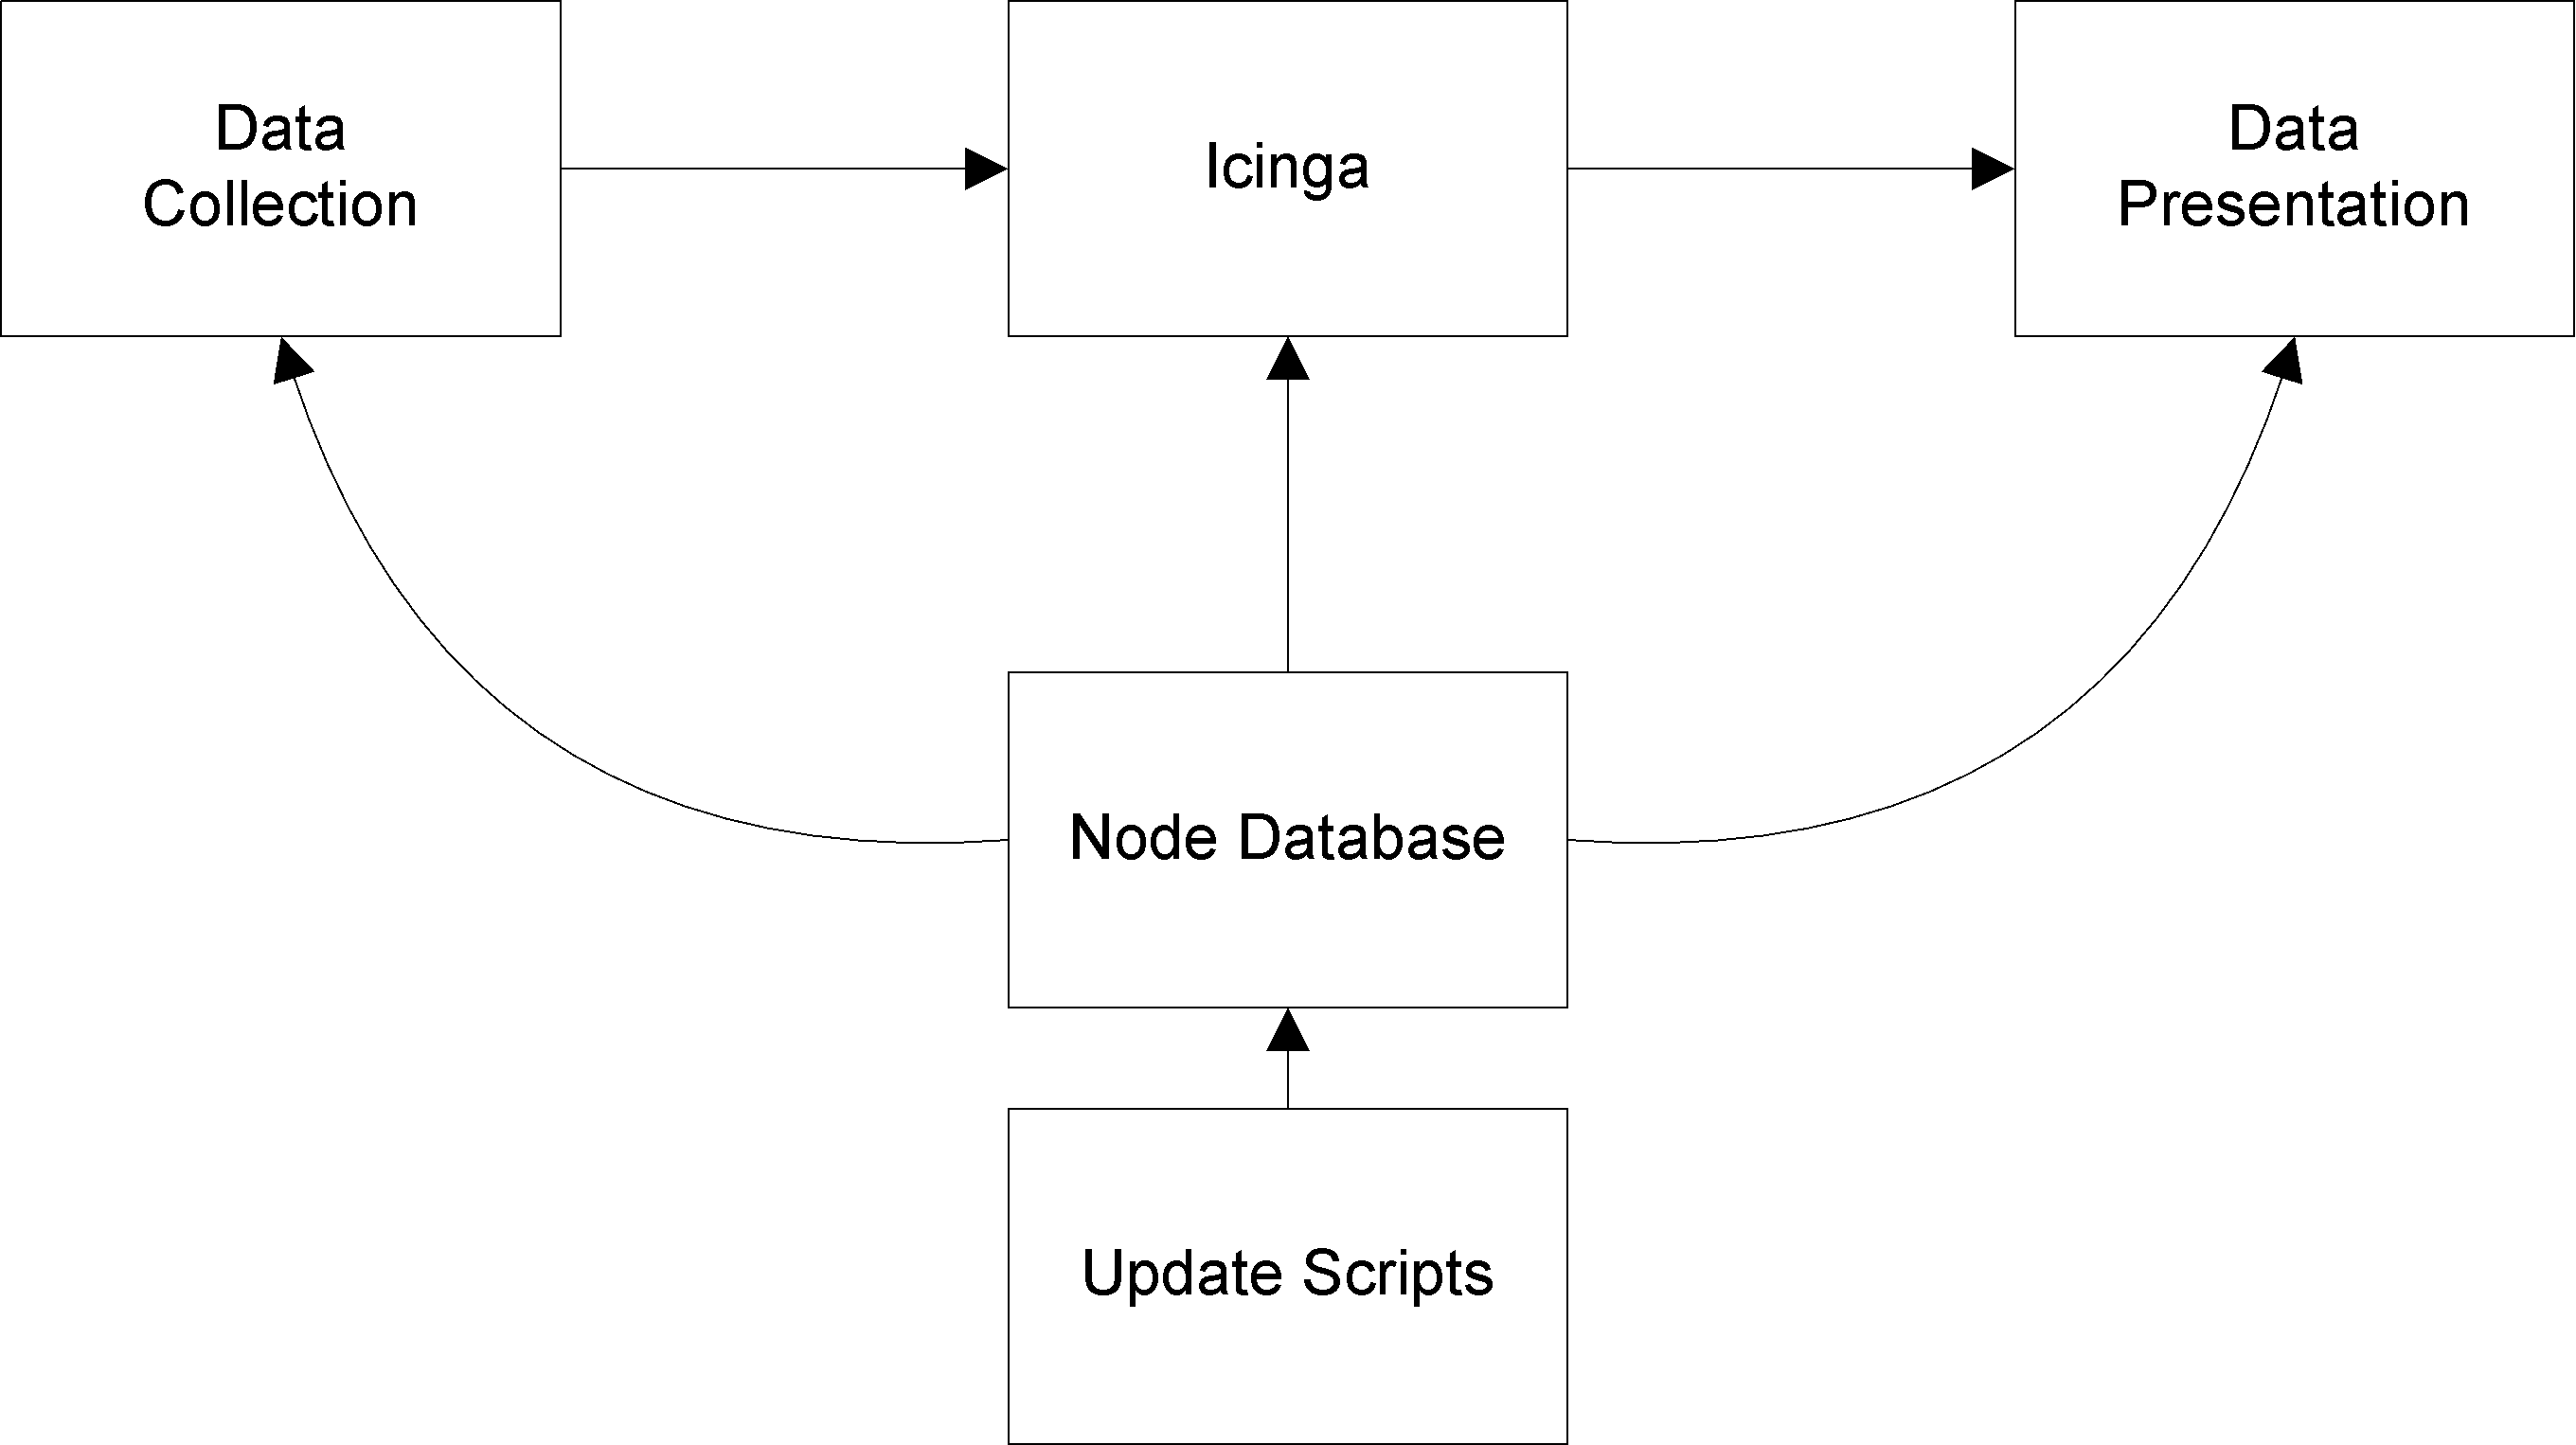
\includegraphics[width=0.7\textwidth]{img/impl-structure.png}
\caption{How the Node Database interfaces with other subsystems}
\label{fig:node-struct}
\end{figure}

\subsubsection{Presentation of Data}

\begin{figure}[htb]
\centering
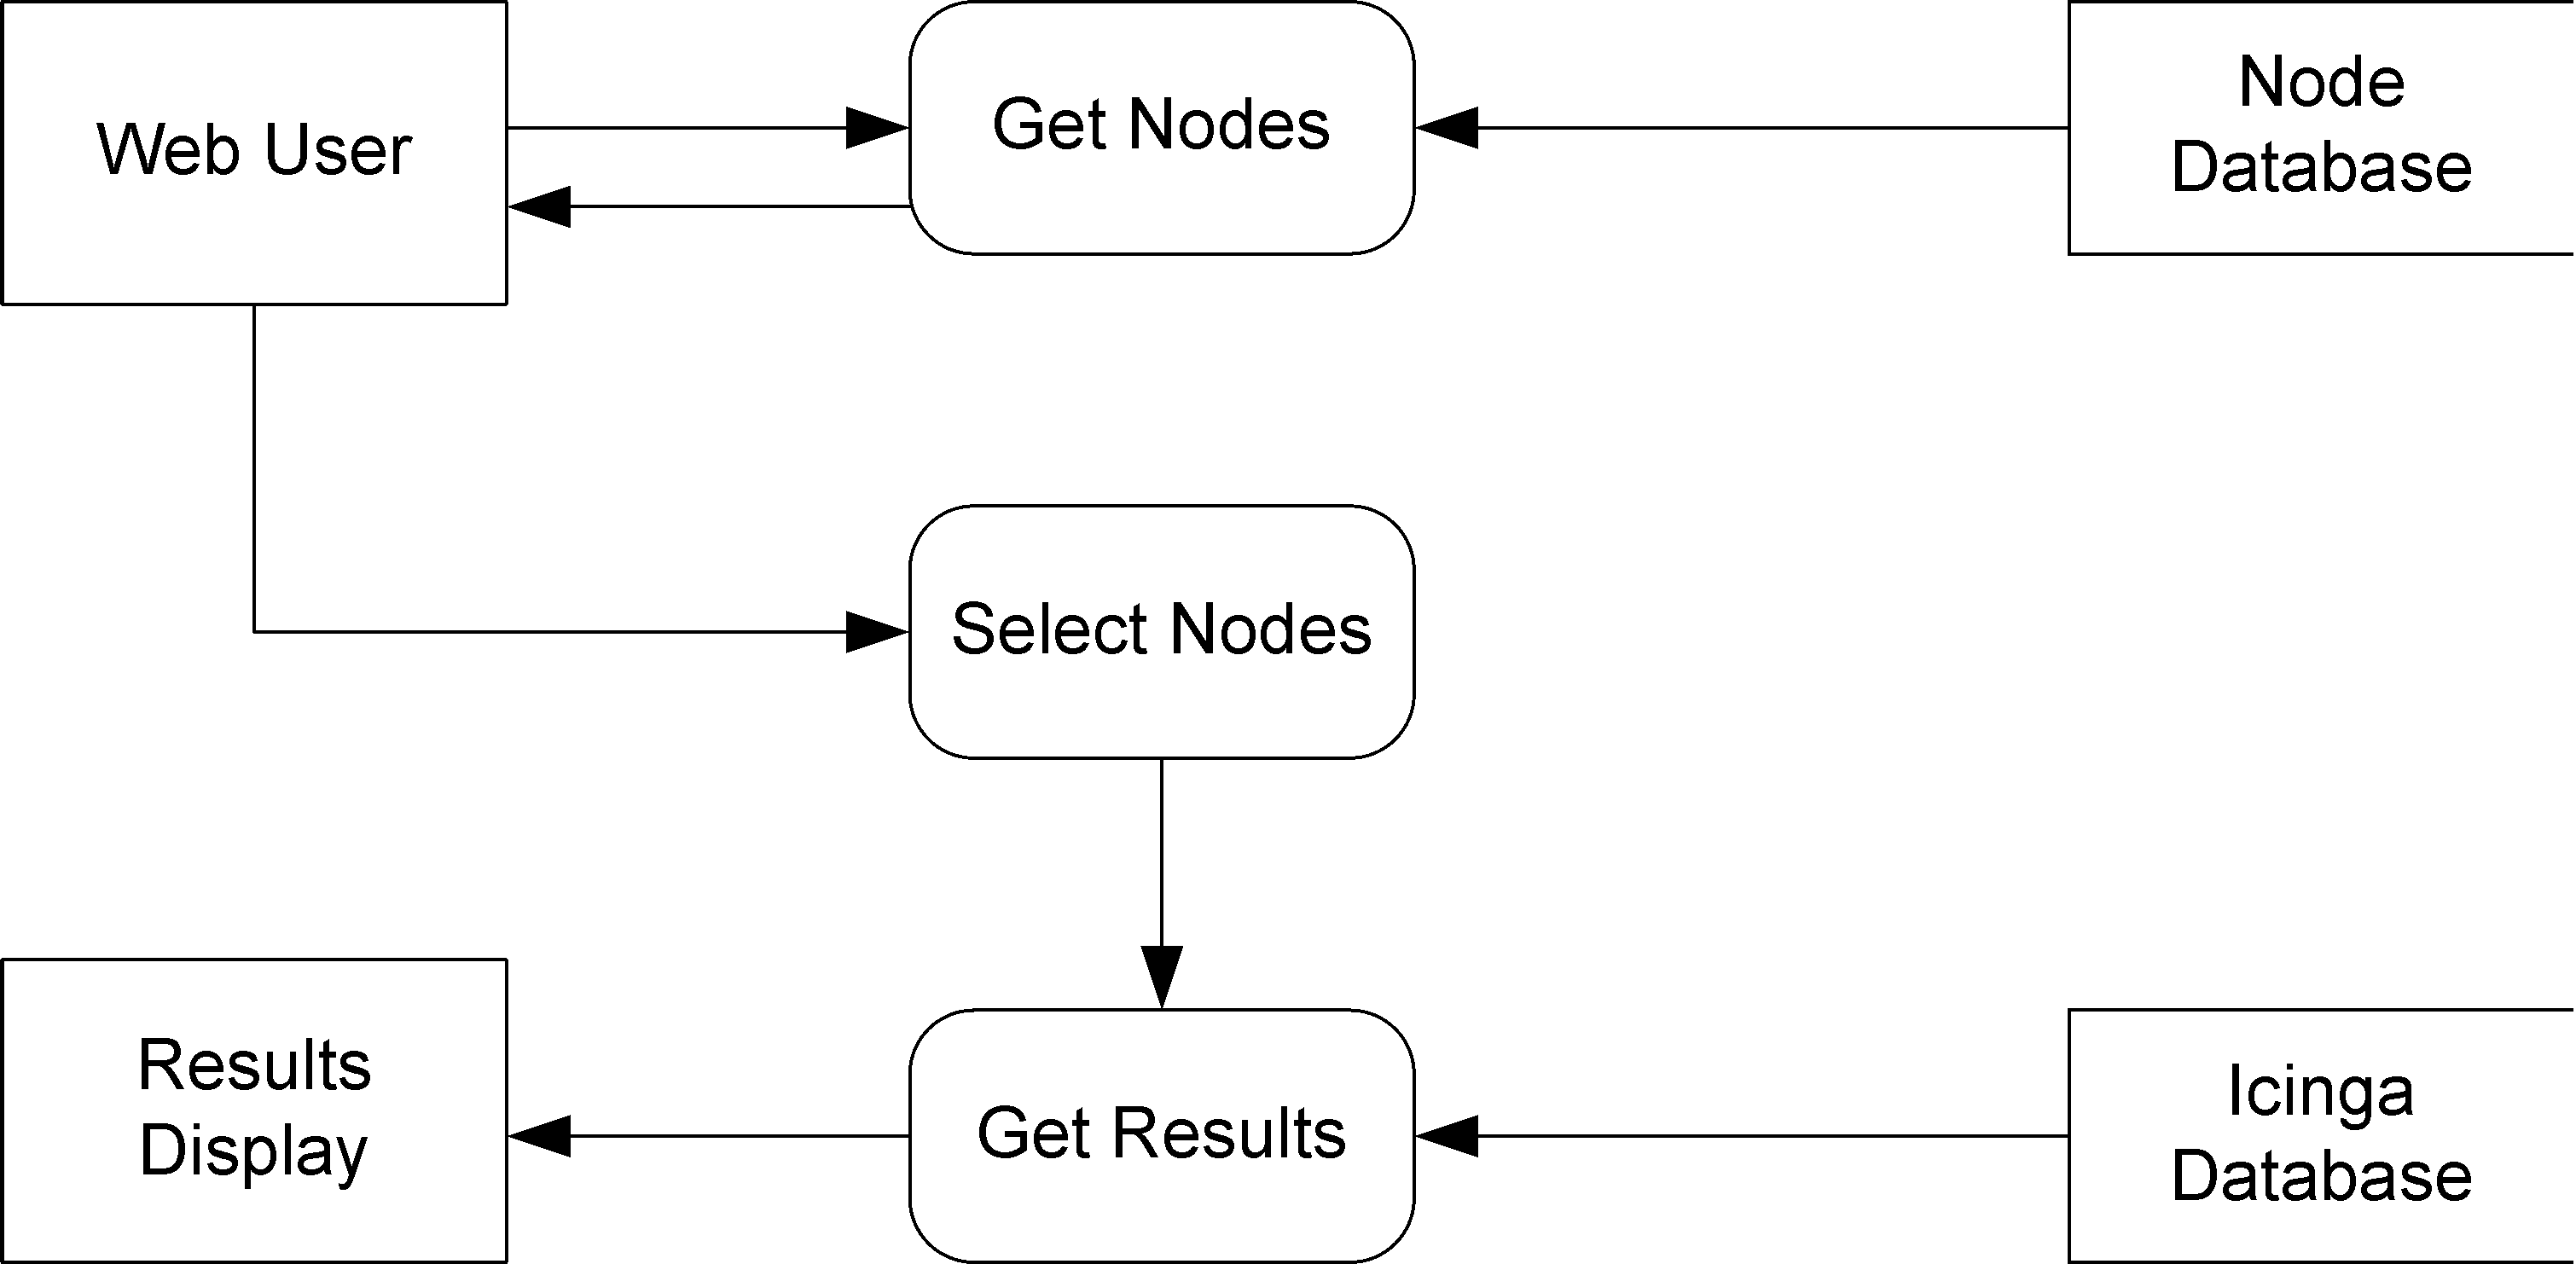
\includegraphics[width=0.8\textwidth]{img/web-dfd.png}
\caption{Data Flow Diagram for the Web Interface}
\label{fig:web}
\end{figure}

